%% =========================================================================
%%  Core Signatures and Inversions --- Wilmott magazine version
%%
%%  Compact practitioner-targeted variant of CoreSignaturesAndInversions_2026.tex.
%%  ~12 pages.  Differences from the full version:
%%
%%    - PBW/Radford derivation compressed to one paragraph + citation chain
%%      (full derivation lives in the arXiv version)
%%    - Lemma 4 (Duval) folded into one sentence
%%    - "On the name Fréchet" Remark replaced with footnote
%%    - Some structural remarks dropped; the substantive ones kept
%%    - Intro leads with the term-structure motivation rather than rough paths
%%    - Theorem environments retained but proofs reduced or pointed to the
%%      companion arXiv preprint
%% =========================================================================

\documentclass[11pt,english]{article}
\usepackage[T1]{fontenc}
\usepackage[utf8]{inputenc}
\usepackage[table]{xcolor}
\usepackage{colortbl}
\usepackage{babel}
\usepackage{cprotect}
\usepackage{float}
\usepackage{url}
\usepackage{amsmath}
\usepackage{amssymb}
\usepackage{amsthm}
\usepackage{graphicx}
\usepackage[a4paper]{geometry}
\geometry{verbose,tmargin=2.5cm,bmargin=2.5cm,lmargin=2.5cm,rmargin=2.5cm,footskip=1cm}
\usepackage{fancyhdr}
\pagestyle{fancy}
\usepackage[pdfusetitle,
 bookmarks=true,bookmarksnumbered=false,bookmarksopen=false,
 breaklinks=false,pdfborder={0 0 1},backref=false,colorlinks=false]
 {hyperref}
\hypersetup{colorlinks=true,citecolor=blue}

\makeatletter
\providecommand{\tabularnewline}{\\}
\makeatother

\usepackage{lastpage}
\usepackage{breakcites}
\lhead{}\chead{}\rhead{}
\lfoot{}\cfoot{\thepage\ / \pageref{LastPage}}\rfoot{}
\renewcommand{\headrulewidth}{0pt}
\usepackage{indentfirst}

\makeatletter
\providecommand*{\shuffle}{\mathbin{\mathpalette\shuffle@{}}}
\newcommand*{\shuffle@}[2]{%
  \sbox0{$#1\vcenter{}$}%
  \kern .15\ht0
  \rlap{\vrule height .25\ht0 depth 0pt width 2.5\ht0}%
  \raise.1\ht0\hbox to 2.5\ht0{%
    \vrule height 1.75\ht0 depth -.1\ht0 width .17\ht0
    \hfill
    \vrule height 1.75\ht0 depth -.1\ht0 width .17\ht0
    \hfill
    \vrule height 1.75\ht0 depth -.1\ht0 width .17\ht0}%
  \kern .15\ht0
}
\makeatother

\usepackage{xurl}
\newcommand{\nbfile}[1]{\nolinkurl{#1}}

%% Allow TeX to expand justification in difficult paragraphs rather
%% than letting them bleed into the right margin.
\setlength{\emergencystretch}{3em}

\newtheorem{theorem}{Theorem}
\newtheorem{proposition}[theorem]{Proposition}
\newtheorem{corollary}[theorem]{Corollary}
\newtheorem{conjecture}[theorem]{Conjecture}

\begin{document}

\title{Core Signatures and Inversions}
\author{Marcos Costa Santos Carreira\thanks{marcoscscarreira@gmail.com}}
\date{\today}
\maketitle

\begin{abstract}
Signatures provide a feature representation for paths that respects
concatenation through Chen's identity, but the truncated signature
is redundant: it carries the same information as the much smaller
log signature. We introduce \emph{core signatures}, a subset of the
truncated signature with the same dimension as the log signature and
no change of basis required --- the core entries are read directly
from the signature, and the remaining entries are recovered through
closed-form substitution rules. Structurally, the core entries are
the Lyndon coordinates of the step-$n$ free nilpotent Lie group; this
identification is classical (Reutenauer 1993; Amendola--Friz--Sturmfels
2019) but the algorithmic packaging is new. We then use Chen's identity
to invert a core signature into a piecewise-linear path of two, three,
or more segments that exactly matches the target signature up to a
chosen truncation level. For more than three segments the inversion
takes the form of a weighted nonlinear least-squares regression in
signature space, and we observe (and conjecture rigorously) that
this regression coincides with the optimal $L^{1}$ piecewise-linear
approximant of the target. The accompanying Mathematica code is at
\url{https://github.com/MarcosCarreira/CoreSignatures}; an application
to USD Treasury and Brazilian DI futures curves is in preparation.

\medskip{}
\textit{Keywords}: signatures; log signatures; Lyndon words; signature
inversion; term-structure modelling
\end{abstract}

%% =========================================================================
\section{Introduction}
%% =========================================================================

Term structures --- interest rates, implied volatilities, futures curves
--- are functions of time-to-maturity that practitioners want to compress
into a small number of geometric features. Principal components do
this in the linear regime; signatures generalise the idea in a way
that respects concatenation. For a path $X:[a,b]\to\mathbb{R}^{d}$,
the signature $S(X)_{a,b}$ collects all iterated integrals along
$X$ into a single tensor series; truncated at level $m$, it provides
a finite-dimensional encoding of $X$ that is faithful up to tree-like
equivalence. The truncated signature contains redundancies coming
from the shuffle relations, and the standard remedy is the log signature
--- whose dimension is that of the free nilpotent Lie algebra $\mathfrak{g}^{m}(\mathbb{R}^{d})$,
typically computed in practice through Reizenstein's \texttt{iisignature}
library \cite{iisignature,iisignature 1004,log signatures}.

This paper develops two results aimed at practitioners working with
truncated signatures. First, we identify a subset of the truncated
signature --- the \emph{core signature} --- that has the same dimension
as the log signature but consists of actual signature entries. The
core entries are exactly the entries indexed by Lyndon words on the
alphabet $\{1,\ldots,d\}$, their count is given by Witt's formula,
and the remaining entries are recovered through explicit substitution
rules obtained from the shuffle relations. Second, we use Chen's identity
to invert a core signature into a concatenation of two or three line
segments in the time-ordered case --- the case relevant for term structures
--- and into longer concatenations through a weighted nonlinear least-squares
regression in signature space. We give numerical evidence that this
regression coincides with the optimal $L^{1}$ piecewise-linear approximant
and state the precise norm-equivalence conjecture that would make
the coincidence rigorous.

The structural identification of core entries with Lyndon coordinates
follows from results that are classical in the algebraic-combinatorics
literature (\cite{Reutenauer}, the Lyndon basis theorem and Radford's
theorem) and in the rough-paths literature (\cite{varieties}, the
universal variety $G^{n}(\mathbb{R}^{d})$). Our contribution is therefore
computational packaging --- naming the subset, exhibiting an explicit
shuffle-product elimination that produces it, tabulating the substitution
rules $Q_{m}$, and using these coordinates for Chen-based inversion
--- rather than a new coordinate theorem. For previous signature-inversion
algorithms see \cite{inversion}.

After our 2023 preprint, \cite{macaulay2} introduced a Macaulay2 package
(\texttt{PathSignatures}) whose \texttt{lyndonShuffle} method implements
the same Lyndon-shuffle decomposition that underlies our substitution
rules $Q_{m}$. In their Section 6 they use the term \emph{core signature
tensor} with a different meaning: the signature of a base path that
generates a family by linear transformation, suited to the algebraic
geometry of signature varieties rather than to Chen-based inversion
of individual signatures. The terminology overlap is unfortunate but
the constructions are distinct. A parallel Julia/OSCAR implementation
is in \cite{signaturetensorsjl}.

%% =========================================================================
\section{Signatures}
%% =========================================================================

A path is a continuous map $X:[a,b]\to\mathbb{R}^{d}$ of bounded variation;
we reparametrise to $[0,1]$ when convenient. The signature truncated
at level $m$ is
\begin{equation}
S^{(\leq m)}(X)_{a,b}\;=\;\Bigl(\,1,\;S^{i_{1}},\;S^{i_{1},i_{2}},\;\ldots,\;S^{i_{1},\ldots,i_{m}}\,\Bigr)\,,\qquad i_{k}\in\{1,\ldots,d\}\,,
\end{equation}
with level-$k$ entries
\begin{equation}
S^{i_{1},\ldots,i_{k}}\;=\;\int_{a}^{b}\int_{a}^{t_{k}}\cdots\int_{a}^{t_{2}}dX_{t_{1}}^{i_{1}}\,\cdots\,dX_{t_{k}}^{i_{k}}\,.\label{eq:IteratedIntegral}
\end{equation}
For a single line segment with slopes $(\beta_{1},\ldots,\beta_{d})$
over an interval of length $T$, every entry has a closed form:
\begin{equation}
S^{i_{1},\ldots,i_{k}}\;=\;\frac{\beta_{i_{1}}\cdots\beta_{i_{k}}T^{k}}{k!}\,.\label{eq:LineSignature}
\end{equation}
This is the building block we will use throughout the inversion.

\paragraph{Shuffle product.}
A $(p,q)$-shuffle of two ordered sequences of lengths $p,q$ is an
interleaving that preserves the relative order within each sequence;
$I\shuffle J$ denotes the multiset of all shuffles of multi-indices
$I$ and $J$. The fundamental shuffle identity --- valid for any
path --- is
\begin{equation}
S^{I}\cdot S^{J}\;=\;\sum_{K\in\,I\shuffle J}S^{K}\,.\label{eq:ShuffleProduct}
\end{equation}
Equation \eqref{eq:ShuffleProduct} is the algebraic engine of Section
\ref{sec:Core}: it provides the relations that reduce the truncated
signature to its core.

\paragraph{Chen's identity.}
For consecutive paths $X:[a,b]\to\mathbb{R}^{d}$ and $Y:[b,c]\to\mathbb{R}^{d}$,
the concatenation $Z=X*Y$ has signature
\begin{equation}
S(Z)_{a,c}\;=\;S(X)_{a,b}\otimes S(Y)_{b,c}\,,\quad\text{or componentwise}\quad z_{i_{1},\ldots,i_{k}}\;=\;\sum_{j=0}^{k}x_{i_{1},\ldots,i_{j}}\cdot y_{i_{j+1},\ldots,i_{k}}\,,\label{eq:ChenIndex}
\end{equation}
with the conventions $x_{\emptyset}=y_{\emptyset}=1$. The componentwise
form allows us to compute individual entries of $Z$ without rebuilding
the full concatenated signature --- the basis of the inversion algorithm
in Section \ref{sec:Inversion}.

%% =========================================================================
\section{Core Signatures\label{sec:Core}}
%% =========================================================================

The shuffle relations mean that not every entry of the truncated signature
carries new information. The standard parsimonious encoding is the
log signature, but it requires a change of basis (specifically, a
Hall-basis projection of the Lie series). We show that a subset of
the truncated signature itself --- the \emph{core elements} --- has
the same dimension and the same information content as the log signature,
can be read directly from $S(X)$, and admits an explicit structural
characterisation in terms of Lyndon words.

\subsection{Core variables via the shuffle product}

Let $V_{m}=\{s_{w}:|w|=m\}$ denote the set of signature entries at
level $m$, and let $C_{m}$ be the \emph{core set up to level} $m$,
defined inductively as the entries that cannot be expressed in terms
of lower-indexed and lower-level entries via the shuffle relations.
For $d=2$, the recursive application of \eqref{eq:ShuffleProduct}
at level 3 produces the Gröbner basis
\[
\begin{array}{l}
3s_{1,1,1}-s_{1}s_{1,1}\,,\quad-s_{2}s_{1,1}+s_{1}s_{2,1}+s_{1,1,2}-s_{2,1,1}\,,\\
-s_{1}s_{2,1}+s_{1,2,1}+2s_{2,1,1}\,,\quad-s_{2}s_{1,2}+s_{2}s_{2,1}+2s_{1,2,2}-2s_{2,2,1}\,,\\
-s_{2}s_{2,1}+s_{2,1,2}+2s_{2,2,1}\,,\quad3s_{2,2,2}-s_{2}s_{2,2}\,.
\end{array}
\]
After eliminating six variables in terms of $C_{2}=\{s_{1},s_{2},s_{1,2}\}$
and the lex-minimal representatives of each remaining orbit, two entries
remain free:
\[
C_{3}\;=\;C_{2}\,\cup\,\{s_{1,1,2},\,s_{1,2,2}\}\,.
\]
Repeating the construction at higher levels yields the core sizes
for $d=2$:
\begin{equation}
|C_{m}|\,\text{ for }m=1,\ldots,6\;=\;2,\,3,\,5,\,8,\,14,\,23\,,\label{eq:CoreSizesD2}
\end{equation}
matching the log-signature column of Reizenstein's tables. For $d=3$
we obtain $3,6,14,32,80,196$, again matching the log signature. The
Lyndon multi-indices that constitute $C_{4},C_{5},C_{6}$ are listed
in Appendix \ref{app:Q}; the substitution rules $Q_{m}$ for $m\leq5$
are tabulated there in full, and $Q_{6}$ for $d\in\{2,3\}$ is exported
in the companion notebook \nbfile{CoreSignatures202412.nb}.

\begin{table}[H]
\centering
\begin{tabular}{|r|r|r|r|r|r|r|}
\hline
$m$ & $d=2$ sig & $d=2$ core/log & $d=3$ sig & $d=3$ core/log & $d=4$ sig & $d=4$ core/log\tabularnewline
\hline\hline
1 & 2 & 2 & 3 & 3 & 4 & 4\tabularnewline\hline
2 & 6 & 3 & 12 & 6 & 20 & 10\tabularnewline\hline
3 & 14 & 5 & 39 & 14 & 84 & 30\tabularnewline\hline
4 & 30 & 8 & 120 & 32 & 340 & 90\tabularnewline\hline
5 & 62 & 14 & 363 & 80 & 1364 & 294\tabularnewline\hline
6 & 126 & 23 & 1092 & 196 & 5460 & 964\tabularnewline\hline
\end{tabular}
\caption{Sizes of signatures and core signatures at low levels. Core sizes
coincide with the log-signature sizes of \cite{log signatures}.\label{tab:Sizes}}
\end{table}

\subsection{Core elements as Lyndon coordinates}

The numerical coincidence $|C_{m}|=\dim\mathfrak{g}^{m}(\mathbb{R}^{d})$
and the choice of the lex-minimal representative in each shuffle orbit
are consequences of the Lyndon basis of the free Lie algebra. Fix
the lexicographic order on $\mathcal{A}=\{1,\ldots,d\}$; a non-empty
word $w$ is a \emph{Lyndon word} if $w<vu$ for every non-trivial
factorisation $w=uv$. For $d=2$, the Lyndon words of length $\leq6$
on $\{1,2\}$ are listed in Table \ref{tab:Lyndon-d2}; comparison
with $C_{6}$ shows the multi-indices agree exactly.

\begin{table}[H]
\centering
\begin{tabular}{|c|l|}
\hline
Length & Lyndon words on $\{1,2\}$\tabularnewline
\hline\hline
1 & $1$, $2$\tabularnewline\hline
2 & $12$\tabularnewline\hline
3 & $112$, $122$\tabularnewline\hline
4 & $1112$, $1122$, $1222$\tabularnewline\hline
5 & $11112$, $11122$, $11212$, $11222$, $12122$, $12222$\tabularnewline\hline
6 & $111112$, $111122$, $111212$, $111222$, $112122$, $112212$, $112222$, $121222$, $122222$\tabularnewline\hline
\end{tabular}
\caption{Lyndon words on $\{1,2\}$ up to length 6. These are exactly the multi-indices
of the core variables.\label{tab:Lyndon-d2}}
\end{table}

\begin{proposition}[Core variables are Lyndon coordinates]
\label{prop:core-is-lyndon} The core sets $C_{m}$ identified by
the shuffle-product computation are exactly the Lyndon words on $\{1,\ldots,d\}$
of length $\leq m$. The corresponding $\sigma_{w}$ form a transcendence
basis for the coordinate ring of the universal variety $G^{m}(\mathbb{R}^{d})$,
and the substitution rules $Q_{m}$ are the explicit form of the corresponding
Radford isomorphism truncated at level $m$.
\end{proposition}

The proof uses three classical ingredients: the Lyndon basis theorem
for the free Lie algebra (\cite{Reutenauer} Theorem 5.1), Poincaré--Birkhoff--Witt,
and Radford's theorem that the shuffle algebra is the free commutative
algebra on Lyndon words (\cite{Reutenauer} Theorem 6.1). Together
they identify the Lyndon-indexed signature entries with algebraically
independent coordinates on the universal variety $G^{n}(\mathbb{R}^{d})$
studied in \cite{varieties}; the lex-minimal choice within each shuffle
orbit corresponds to the Lyndon representative by Duval's factorisation
theorem (\cite{Reutenauer} Theorem 5.1.5). The full derivation is
given in the companion arXiv preprint.

\subsection{Witt formula and the Pascal-triangle structure}

The number of Lyndon words of length $n$ on a $d$-letter alphabet
is given by Witt's formula (\cite{Reutenauer} Section 4):
\begin{equation}
\ell_{d}(n)\;=\;\frac{1}{n}\sum_{k\,\mid\,n}\mu\!\left(\tfrac{n}{k}\right)\,d^{\,k}\,,\label{eq:Witt}
\end{equation}
where $\mu$ is the Möbius function. For $d=2$ this gives the sequence
$2,1,2,3,6,9,18,30,\ldots$ whose cumulative sums match \eqref{eq:CoreSizesD2}.
The multi-graded refinement of \eqref{eq:Witt} --- counting Lyndon
words on $\{1,2\}$ with prescribed numbers of $1$s and $2$s --- recovers
the Pascal-triangle distribution we observed empirically in the substitution
rules.

%% =========================================================================
\section{Inversion of Core Signatures\label{sec:Inversion}}
%% =========================================================================

We use Chen's identity \eqref{eq:ChenIndex} to recover, from a target
core signature, a piecewise-linear path whose own core signature exactly
matches the target up to a chosen truncation level. We treat the time-ordered
case $X(t)=(t,f(t))$ in detail --- this is the case relevant for
term structures --- and outline the general 2d case at the end.

\paragraph{Related work on the inversion problem.}
Three recent papers from the Berlin/TU group develop the inversion
problem from an algebraic-geometric angle that complements ours. \cite{splines}
generalise the piecewise-linear and polynomial classes of \cite{varieties}
to piecewise polynomial paths and splines, and introduce the \emph{path
recovery degree} (Definition 6.1) as the number of complex points
in a generic fibre of the signature map: the formal counterpart of
our empirical observation that the two-piece time-ordered system has
two solutions. For $d=2$ at level $k=4$, their Table 3 records the
recovery degree as $4$ for piecewise linear paths with four segments
and up to $40$ for higher-degree spline classes. \cite{tensorlearning}
gives an $O(d^{4})$ algorithm for the level-3 $d$-segment piecewise
linear case using Gauss transformations on signature tensors as a
tensor analogue of congruence normal forms, outperforming Gröbner-basis
methods. \cite{barycenters} treats the adjacent problem of path recovery
from \emph{barycenters} of multiple signatures, relevant when the
input is an expected signature.

We develop the time-ordered case $X(t)=(t,f(t))$ in detail because
the algebra closes with closed-form Chen-identity solutions for two
and three segments (Appendix \ref{app:Q}), and because this is the
case most relevant for term structures; the same machinery extends
to general two-dimensional paths --- see the semicircle and digit-5
examples below --- and in principle to higher dimensions. For multi-piece
inversion we use a weighted regression in signature space whose moment-matching
interpretation, via the Lyndon coordinates of Section \ref{sec:Core},
links signature-space minimisation to classical $L^{1}$ approximation
theory --- a connection that is, to our knowledge, not present in
the algebraic-geometric line of work above.

\subsection{Time-ordered paths: two pieces}

Let $X(t)=(t,f(t))$ on $[0,T]$. We seek a concatenation $X*Y$ of
two line segments
\[
X(t)|_{[0,t_{1}]}=(t,\beta_{1}t)\,,\qquad Y(t)|_{[t_{1},T]}=(t,\beta_{1}T+\beta_{2}t)\,,
\]
parametrised by $\{T,t_{1},\beta_{1},\beta_{2}\}$, whose core signature
matches a target $\{z_{1},z_{2},z_{1,2},z_{1,1,2},z_{1,2,2}\}$. By
\eqref{eq:LineSignature} and \eqref{eq:ChenIndex}, the matching conditions
are the five equations of Table \ref{tab:SystemChenTS2P}.

\begin{table}[H]
\centering
\begin{tabular}{|r|r|l|}
\hline
Level & Eq \# & Equation\tabularnewline\hline\hline
1 & 1 & $T=z_{1}$\tabularnewline\hline
1 & 2 & $\beta_{1}t_{1}+\beta_{2}(T-t_{1})=z_{2}$\tabularnewline\hline
2 & 3 & $\frac{1}{2}\beta_{1}t_{1}^{2}+\frac{1}{2}\beta_{2}(T-t_{1})^{2}+\beta_{2}t_{1}(T-t_{1})=z_{1,2}$\tabularnewline\hline
3 & 4 & $\frac{1}{6}\beta_{1}t_{1}^{3}+\frac{1}{6}\beta_{2}(T-t_{1})^{3}+\frac{1}{2}\beta_{2}t_{1}(T-t_{1})^{2}+\frac{1}{2}\beta_{2}t_{1}^{2}(T-t_{1})=z_{1,1,2}$\tabularnewline\hline
3 & 5 & $\frac{1}{6}\beta_{1}^{2}t_{1}^{3}+\frac{1}{6}\beta_{2}^{2}(T-t_{1})^{3}+\frac{1}{2}\beta_{2}^{2}t_{1}(T-t_{1})^{2}+\frac{1}{2}\beta_{1}\beta_{2}t_{1}^{2}(T-t_{1})=z_{1,2,2}$\tabularnewline\hline
\end{tabular}
\caption{System for the two-piece time-ordered inversion.\label{tab:SystemChenTS2P}}
\end{table}

The system has five equations in four unknowns and admits two solutions,
obtained by dropping equation $\#5$ or equation $\#4$; the closed
forms are in the companion notebook, and substituting either solution
into the dropped equation gives the consistency condition
\begin{equation}
2z_{1,2}^{2}+z_{1}z_{2}z_{1,2}\;=\;3z_{1}z_{1,2,2}+3z_{2}z_{1,1,2}\,,
\end{equation}
which expresses the algebraic limit of two segments.

\paragraph{Worked examples.}
\begin{sloppypar}
For $f(t)=\sin(\pi t)$ on $[0,1]$, the target core signature is
$\{1,0,-2/\pi,-1/\pi,1/4\}$. Solution 1 (dropping equation $\#5$)
gives the symmetric tent with peak $(1/2,4/\pi)$. For $f(t)=\sin(\pi t^{2})$
Solution 1 gives an asymmetric tent with peak slightly past $t=1/2$,
matching the geometric asymmetry of the curve (Figure \ref{fig:sint12l2}).
For $f(t)=\sin(\pi t^{2})+1-t$ both solutions exist and produce two
two-segment fits whose crossing point sits very close to the original
curve (Figure \ref{fig:sint21tl2}); the two values of $t_{1}$ bracket
the location of maximum curvature.
\end{sloppypar}

\begin{figure}[H]
\centering
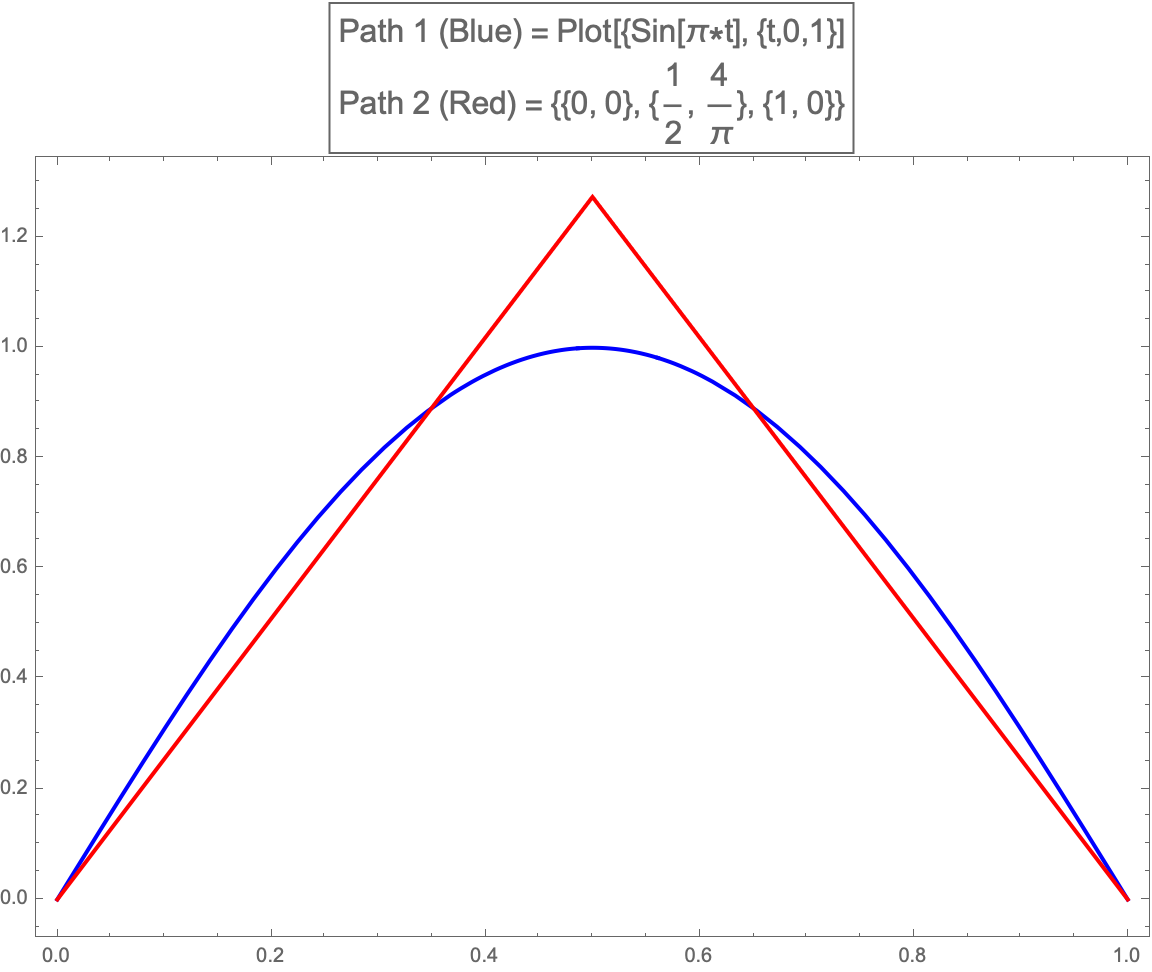
\includegraphics[scale=0.45]{figures/FitSint1l2}\hfill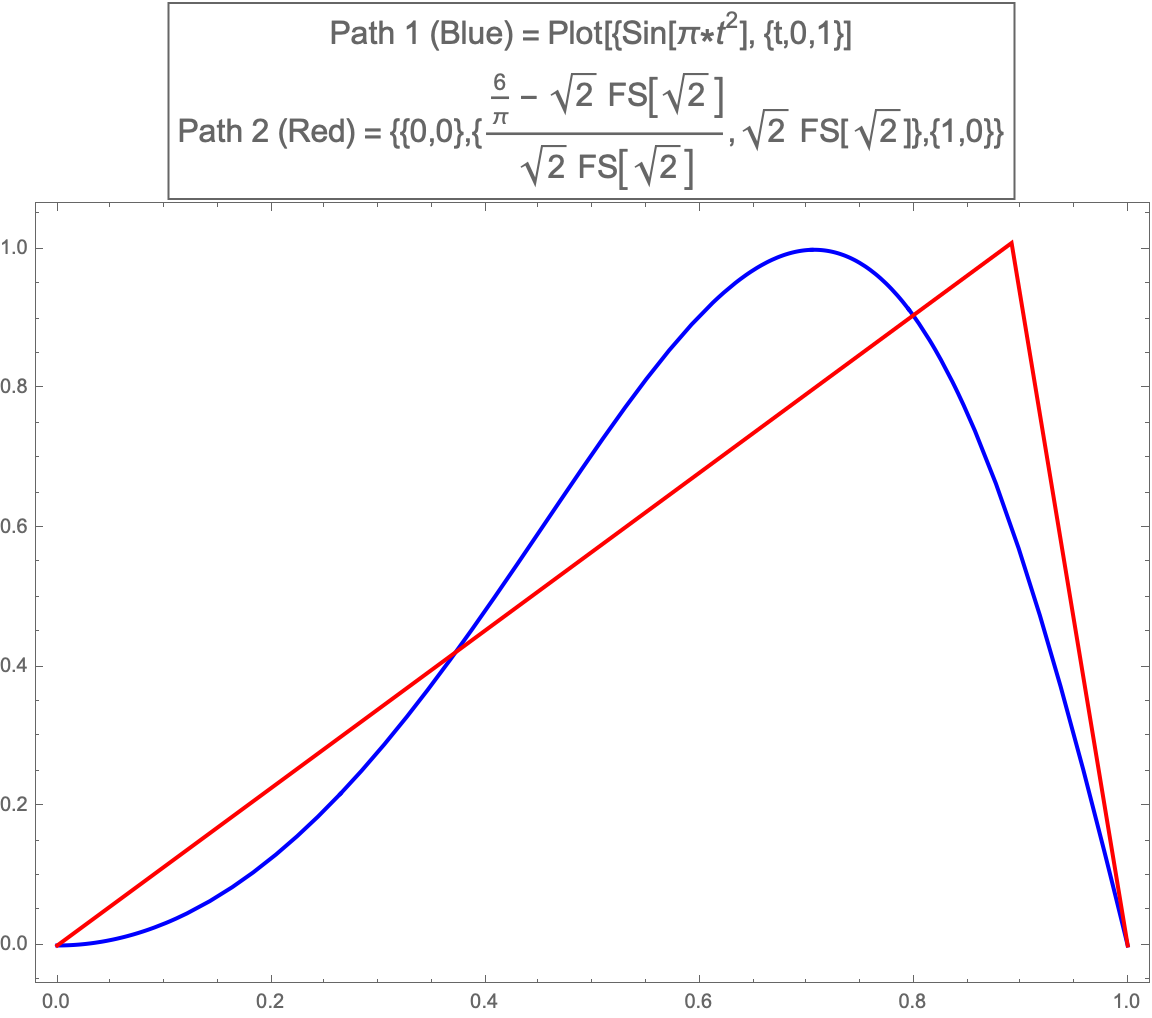
\includegraphics[scale=0.45]{figures/FitSint2l2}
\caption{Two-segment fits to $\{t,\sin(\pi t)\}$ (left) and $\{t,\sin(\pi t^{2})\}$
(right).\label{fig:sint12l2}}
\end{figure}

\begin{figure}[H]
\centering
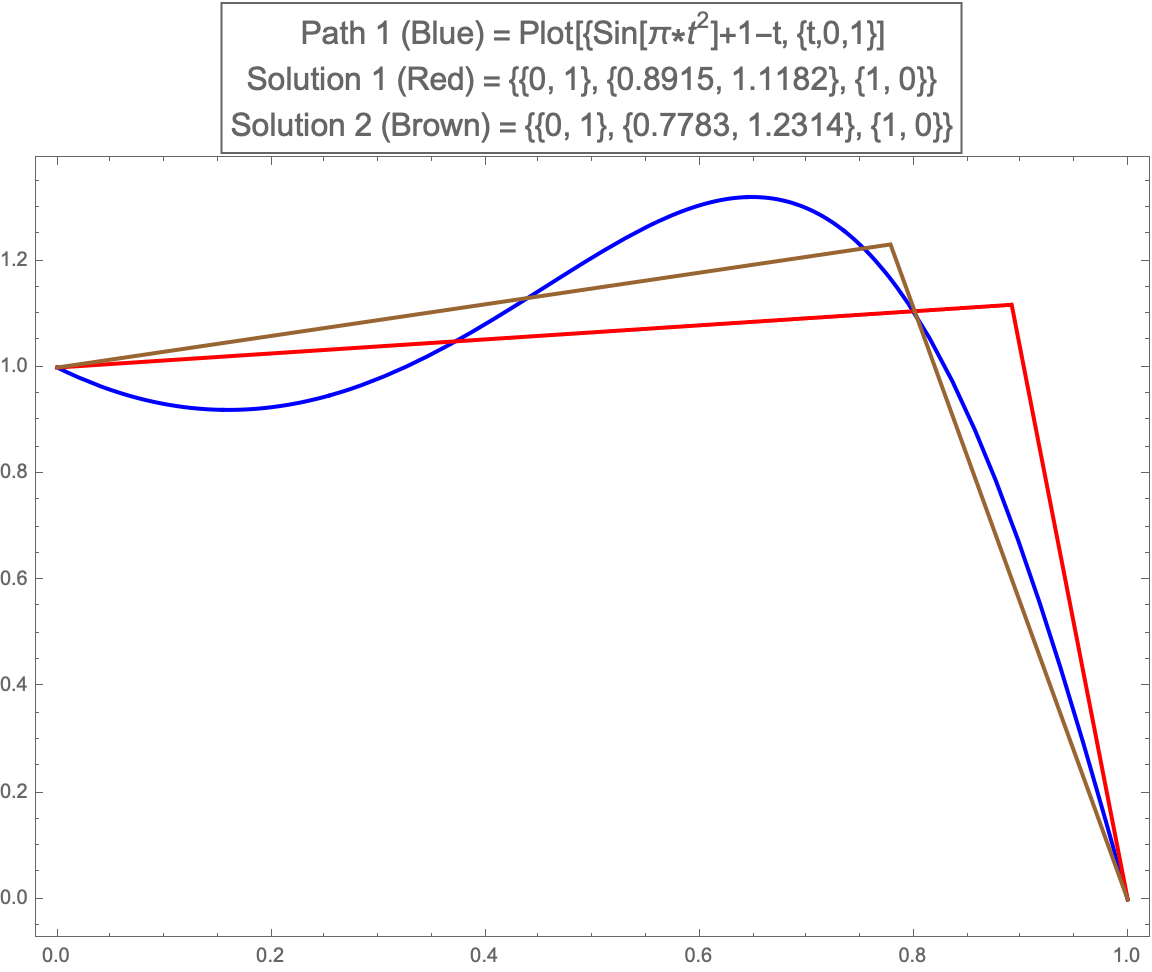
\includegraphics[scale=0.45]{figures/FitSint21tl2}
\caption{The two two-segment fits to $\{t,\sin(\pi t^{2})+1-t\}$.\label{fig:sint21tl2}}
\end{figure}

\subsection{Adversarial cases and three pieces}

The two-piece inversion fails when $z_{1}z_{2}-2z_{1,2}=0$ (Lévy
area zero relative to the chord) or when $z_{2}=0$ removes one of
the two solutions. Both situations occur for $\{t,\sin(2\pi t)\}$
and similar oscillatory targets. The remedy is to add a third segment;
the extended system has three more unknowns and four more equations
from level 4 and the cross-terms (full listing in the companion notebook,
section \texttt{ThreePiece}), with the same overdetermined-Gröbner
structure and its own closed-form solutions for each choice of dropped
equation.

\subsection{Four or more pieces, and the regression formulation}

For four or more segments the algebraic Gröbner approach becomes prohibitively
expensive. The practical alternative is a nonlinear weighted least-squares
regression in signature space: with $\theta$ parameterising the piecewise-linear
path and $\mathcal{L}_{m}$ the set of Lyndon words up to level $m$,
\begin{equation}
\theta^{\star}\;=\;\underset{\theta}{\arg\min}\;\sum_{w\in\mathcal{L}_{m}}w_{w}\bigl(\sigma_{w}[g_{\theta}]-\sigma_{w}[X]\bigr)^{2}\,.\label{eq:weighted-regression}
\end{equation}
The companion notebook uses level-only weights $w_{w}=W_{|w|}$ with
$W_{\bullet}=\{50,50,30,10,10,3,3,3\}$ across the core indices and
\texttt{DifferentialEvolution} as the optimiser. Signature entries
at level $k$ on a path of duration $T$ scale as $O(T^{k}/k!)$ via
the simplex of integration, so the weights are decreasing with level
to keep all residuals on comparable footing.

Figures \ref{fig:sinpaths4pts}--\ref{fig:digit5_5} show four- and
five-segment fits to oscillatory time-ordered paths, to the semicircle,
and to the digit ``5''. The five-piece digit-5 fit recovers the topology
of the original 7-segment path to visual accuracy.

\begin{figure}[H]
\centering
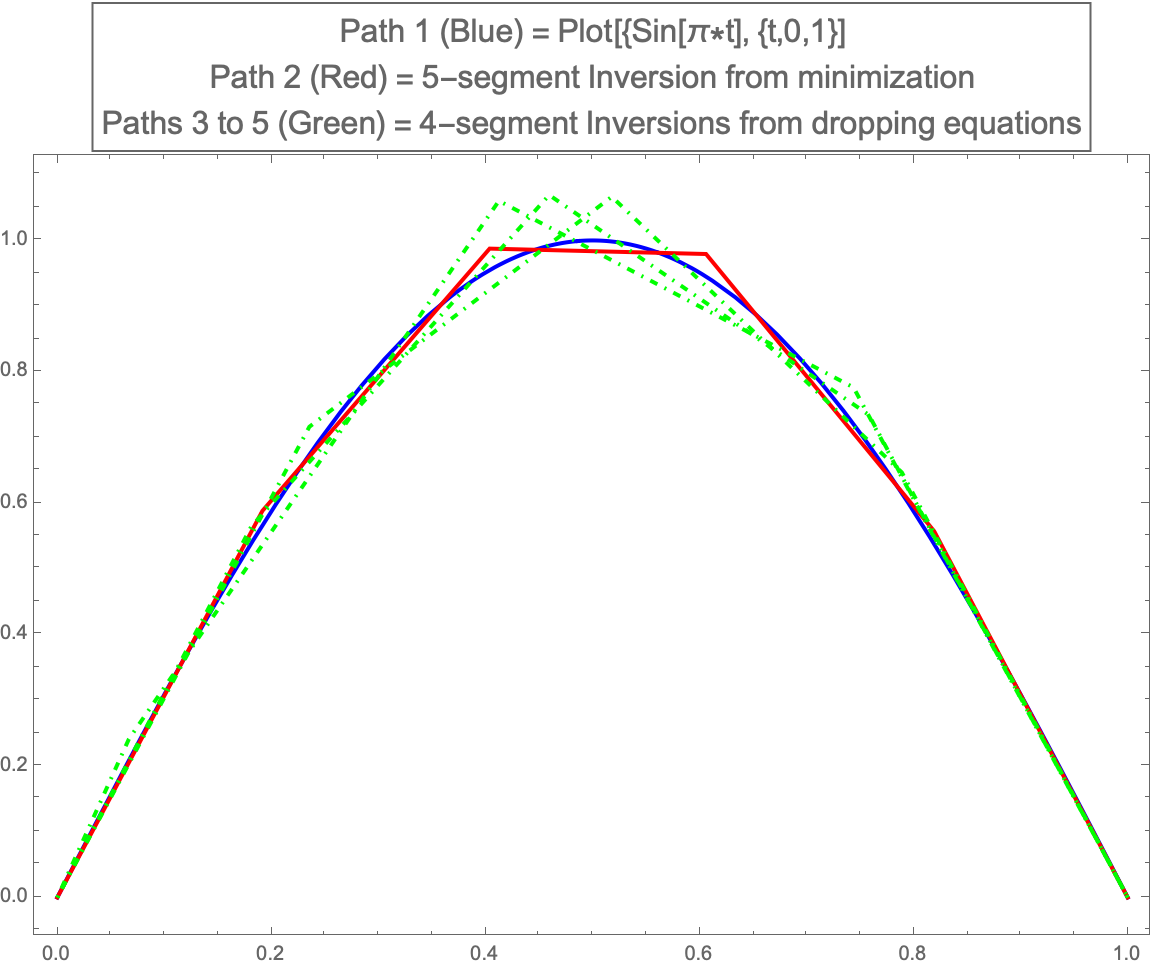
\includegraphics[scale=0.45]{figures/Fit4pPath1}\hfill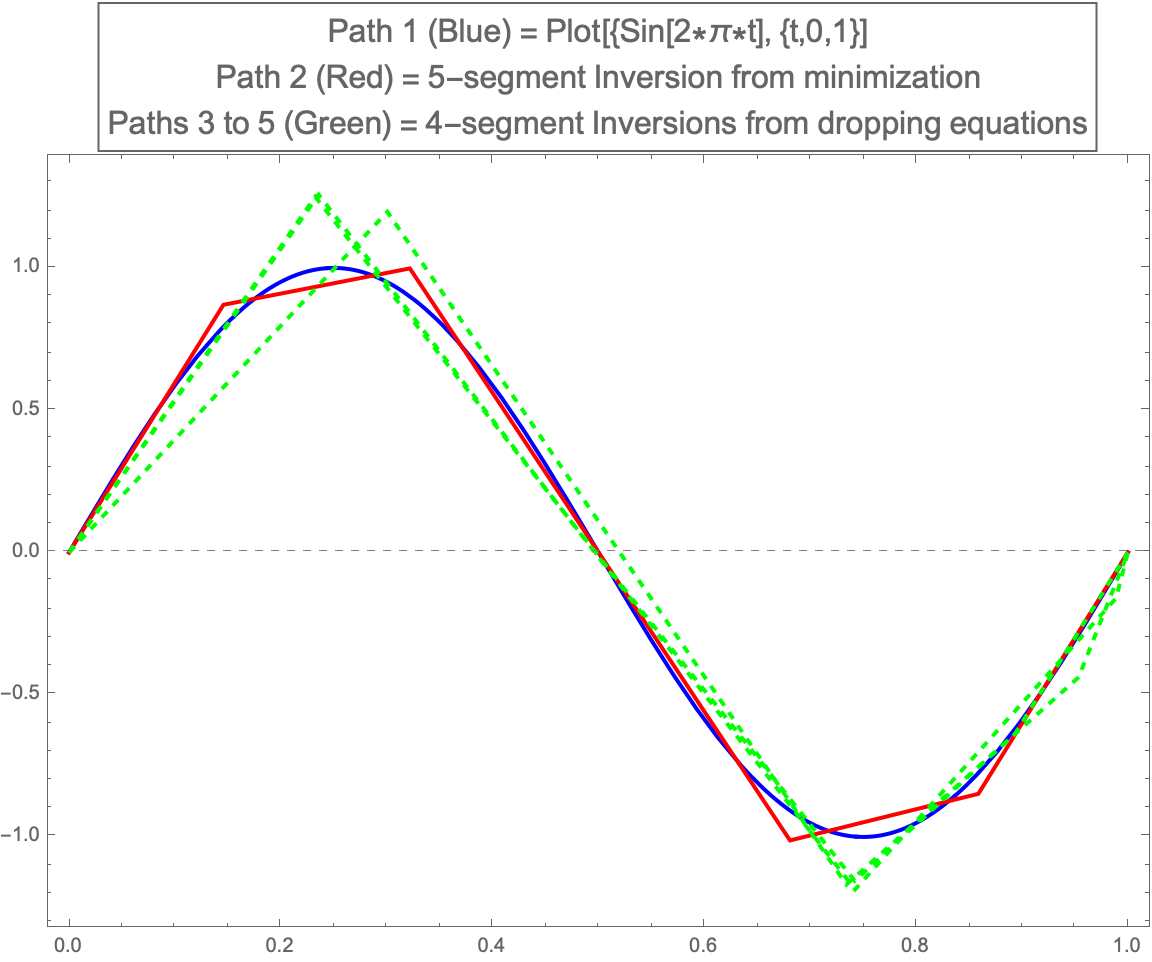
\includegraphics[scale=0.45]{figures/Fit4pPath2}
\caption{Fits of 4 and 5 segments to $\{t,\sin(k\pi t)\}$.\label{fig:sinpaths4pts}}
\end{figure}

\begin{figure}[H]
\centering
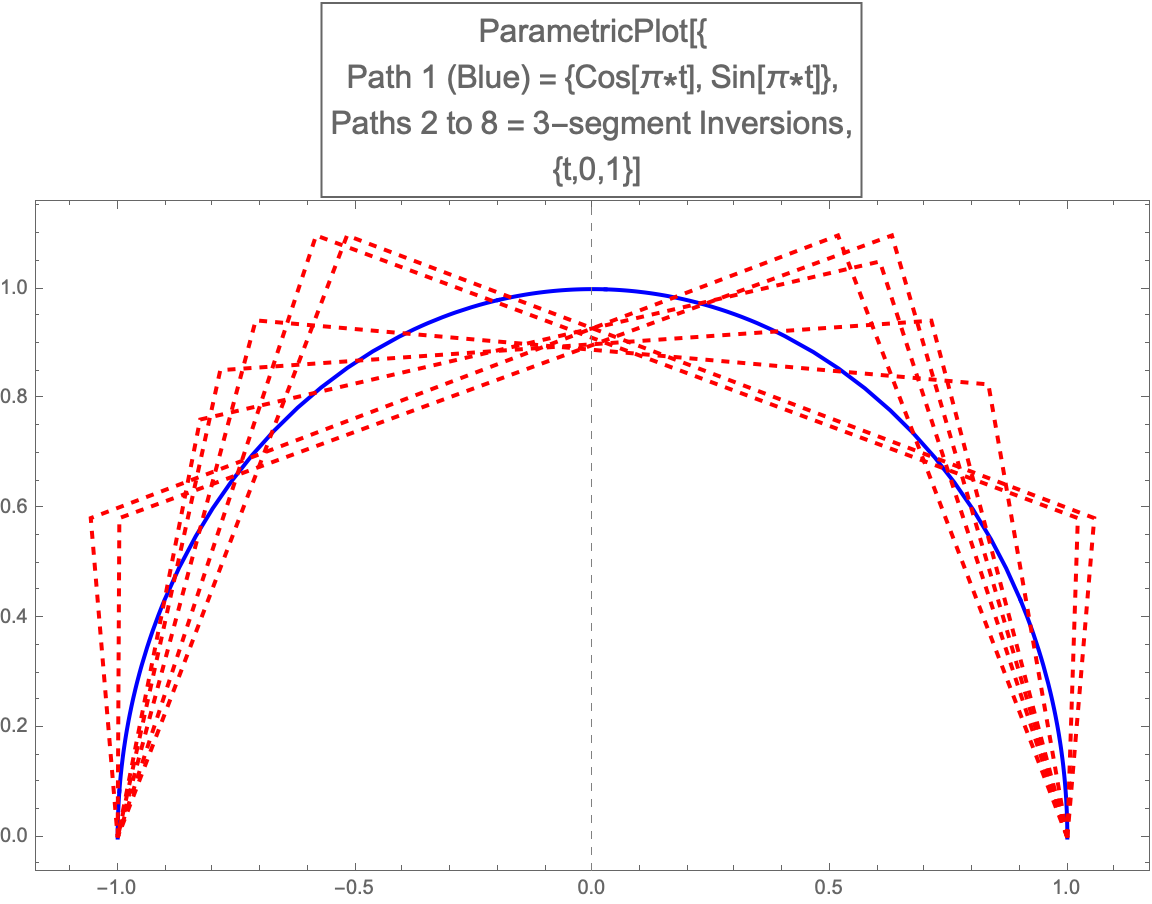
\includegraphics[scale=0.4]{figures/SemiCircle3}\hfill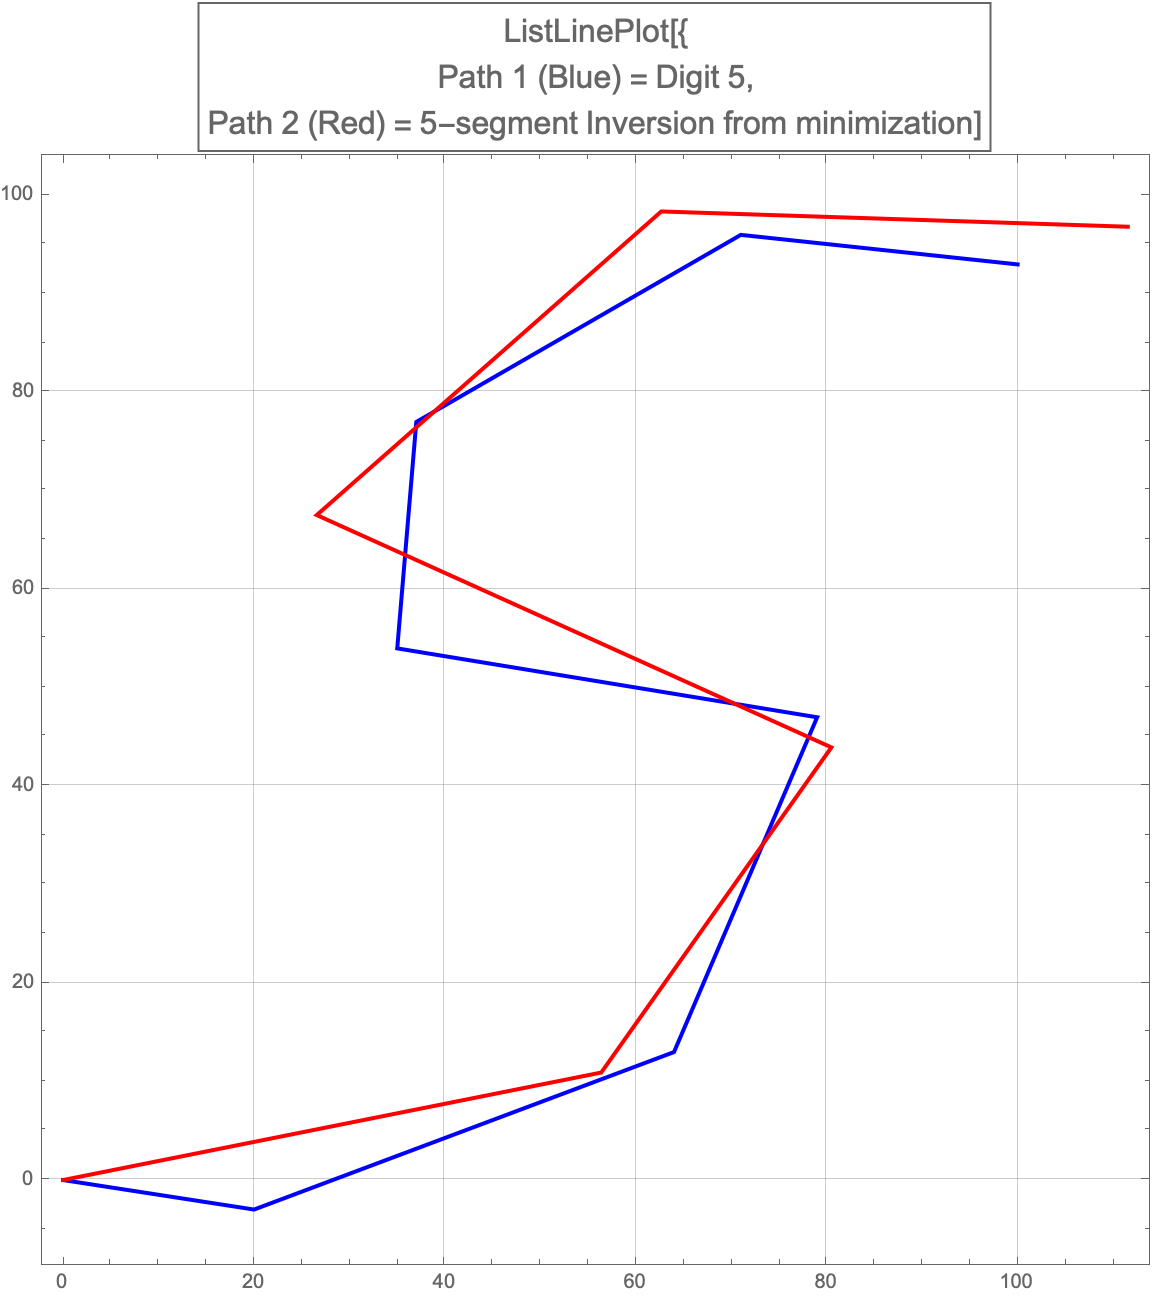
\includegraphics[scale=0.4]{figures/Digit5_5}
\caption{Three-piece inversion of the semicircle (left) and five-segment inversion
of the digit 5 (right).\label{fig:digit5_5}}
\end{figure}

\subsection{Signature entries as iterated path moments}

For $X(t)=(t,f(t))$ on $[0,T]$, integration by parts gives
\[
\sigma_{1,2}[X]=Tf(T)-\int_{0}^{T}f(t)\,dt\,,\qquad\sigma_{1,1,2}[X]=\tfrac{T^{2}}{2}f(T)-\int_{0}^{T}tf(t)\,dt\,,
\]
and analogously for higher Lyndon entries. To leading order in the
level grading, every Lyndon-word signature entry of a time-augmented
path is a polynomial in the moments $M_{k}(f)=\int_{0}^{T}t^{k}f(t)\,dt$
and the boundary values. The regression \eqref{eq:weighted-regression}
is therefore, asymptotically, a weighted moment-matching of $g_{\theta}$
to $f$. The classical Hausdorff moment problem (\cite{Talenti}) then
tells us that matching the first $m$ moments of $f\in C^{s}([0,T])$
pins down $f$ in $L^{1}$ to order $O(m^{-s})$, which is the same
rate one would get from optimal piecewise-polynomial approximation.

We can give that observation quantitative form. The companion notebook
\nbfile{Frechet.nb} runs an evolutionary algorithm on the four-segment
piecewise-linear class minimising the mean pointwise distance%
\footnote{Despite the filename, the objective is not a Fréchet distance: since
both paths share the time coordinate, $\mathrm{EuclideanDistance}\bigl((t,f(t)),(t,g_{\theta}(t))\bigr)=|f(t)-g_{\theta}(t)|$,
so the algorithm is minimising the mean $L^{1}$ error.}
\[
\mathrm{meandist}(g_{\theta},f)\;=\;\tfrac{1}{N+1}\sum_{i=0}^{N}\bigl|f(t_{i})-g_{\theta}(t_{i})\bigr|\,,\qquad t_{i}=iT/N\,.
\]
On the target $f(t)=\sin(2\pi t^{2})$, the mean-$L^{1}$ evolutionary
algorithm and the algebraic core-signature inversion of the preceding
subsections converge to qualitatively similar piecewise-linear approximations,
with interior breakpoints agreeing to within a few percent. The two
algorithms minimise different objectives --- signature-space residual
sum for the algebraic inversion, mean $L^{1}$ distance for the evolutionary
algorithm --- and converge to distinct nearby minima rather than to
a common optimum: the multi-segment analogue of the single-segment
$4.7\%$ obstruction noted below.

\subsection{The norm-equivalence conjecture}

A heuristic explanation for the coincidence is visible: both methods
determine the breakpoints by first-order conditions on identical leading
moments of $f$, differing only by terms of order $\sup|f''|\cdot(\Delta t)^{2}$.
This is an approximation-theoretic intuition rather than a proof of
norm equivalence; we conjecture that the rigorous form is:

\begin{conjecture}[Signature-norm equivalence]
\label{conj:norm-equivalence} For $f,g$ in a class $\mathcal{F}\subseteq C^{1}([0,T];\mathbb{R})$
of paths of bounded derivative, there exist weights $w_{w}$ depending
only on $|w|$ and $T$, with $w_{w}\sim(k!)^{2}/T^{2k}$ for $|w|=k$,
and a Sobolev exponent $s\geq0$ such that
\[
\sum_{w\in\mathcal{L}}w_{w}\bigl(\sigma_{w}[G]-\sigma_{w}[X]\bigr)^{2}\;\asymp\;\|f-g\|_{H^{s}([0,T])}^{2}
\]
uniformly for $f,g$ in compact subsets of $\mathcal{F}$, with constants
of equivalence depending only on the diameter of the compact set in
$H^{s}$.
\end{conjecture}

The conjecture is supported by: (i) the empirical coincidence above
on a finite test set, (ii) the moment-matching identification, and
(iii) the classical link between moment matching and $L^{1}/L^{2}$
approximation. A direct computation on the simplest case --- one free
interior breakpoint $(\tau,y)$ on $[0,T]$ with pinned endpoints ---
shows that the two minimisers do not coincide pointwise: for $f(t)=\sin(\pi t)$,
$T=1$, symmetry forces $\tau^{\star}=1/2$ and the values are $y_{\sigma}=4/\pi\approx1.273$
versus $y_{L^{2}}=12/\pi^{2}\approx1.216$, a 4.7\% discrepancy. The
conjecture is therefore not pointwise identity of minimisers but norm
equivalence in the overdetermined regime, with the constants of equivalence
depending on the smoothness of $f$. The natural first-proof target
is the class of \emph{polynomial paths}, where the universal-variety
coordinates are described explicitly in \cite{varieties} and \cite{learning}
and the moment-matching identities reduce to finite-dimensional linear
systems. An empirical complement is to calibrate the weights $w_{w}$
on representative training sets spanning both \emph{rough paths} (where
level-$k$ entries can saturate the $O(T^{k}/k!)$ bound and the worst-case
scaling $(k!)^{2}/T^{2k}$ is natural) and \emph{smooth targets} (where
the actual entries shrink faster and decreasing weights win on signal-to-noise);
the calibrated asymptotic would identify the smoothness class on which
the simple conjecture holds, versus one requiring a target-dependent
weight scheme.

\paragraph{Concatenation.}
By Chen's identity and the linearity of moments, segment-wise regression
errors compose into a global error bounded by their sum: for a partition
of $[0,T]$ into $N$ pieces $X^{(i)}$ with per-segment approximations
$g^{(i)}$,
\[
\sum_{w\in\mathcal{L}_{m}}w_{w}\bigl(\sigma_{w}[g]-\sigma_{w}[X]\bigr)^{2}\;\leq\;C(m,N)\sum_{i=1}^{N}\sum_{w\in\mathcal{L}_{m}}w_{w}\bigl(\sigma_{w}[g^{(i)}]-\sigma_{w}[X^{(i)}]\bigr)^{2}\,.
\]
A target $f$ of characteristic frequency $\omega_{0}$ then needs
$N\sim\omega_{0}T$ segments of length $\Delta t\sim1/\omega_{0}$
to keep the per-segment level requirement bounded; the global $L^{1}$
error scales as $O(N^{-(m+1)})$ for $f\in C^{m+1}$, matching classical
piecewise-polynomial approximation rates.

\subsection{Dictionary}

The picture this section develops is the following correspondence
between algebraic objects from Section \ref{sec:Core} and approximation-theoretic
objects.

\begin{center}
\begin{tabular}{|l|l|}
\hline
Core-signature inversion & Approximation theory\tabularnewline
\hline\hline
Lyndon coordinates of $G^{n}(\mathbb{R}^{d})$ & Coordinates on the universal variety\tabularnewline\hline
Algebraic exact inversion (Sec.\ \ref{sec:Inversion}) & Galerkin projection in determined regime\tabularnewline\hline
Weighted regression \eqref{eq:weighted-regression} & Sobolev projection (under Conjecture \ref{conj:norm-equivalence})\tabularnewline\hline
Chen concatenation & Additive error decomposition over partition\tabularnewline\hline
Truncation level $m$ & Moment-matching truncation parameter\tabularnewline\hline
\end{tabular}
\par\end{center}

%% =========================================================================
\section{Conclusions and forthcoming work}
%% =========================================================================

We introduced core signatures, identified them structurally with the
Lyndon coordinates of the universal variety $G^{n}(\mathbb{R}^{d})$
(Proposition \ref{prop:core-is-lyndon}), sized them via Witt's formula,
and gave an explicit Gröbner-basis algorithm for the substitution
rules that express any signature entry in core form. We then used
Chen's identity to invert core signatures into piecewise-linear paths
of two, three, or more segments, and reframed the multi-segment case
as a weighted nonlinear least-squares regression in signature space
whose minimiser empirically coincides with the optimal piecewise-linear
$L^{1}$ approximant.

The application of the core-signature framework to interest-rate term
structures is in preparation. The companion paper applies the inversion
to the historical USD Treasury curve and Brazilian DI futures curve
to extract a low-dimensional geometric encoding of curve dynamics
suitable for stress testing, hedging, and historical-pattern recognition
across the two markets. The framework has also been adopted in practitioner
work on quantitative-trading futuretesting; see \cite{bloch_futuretesting}.
We thank Sam Cohen (Oxford) for helpful discussions.

\paragraph{Use of AI assistance.}
The author used Anthropic's Claude to review the mathematical content
of the 2023 version of this paper, tighten the exposition, supply
the theoretical citation chain through the Lyndon basis theorem,
Poincaré--Birkhoff--Witt and Radford's theorem that identifies the
core variables with the Lyndon coordinates of $G^{n}(\mathbb{R}^{d})$,
and help draft the regression and norm-equivalence framing of Sections
4.3--4.5. All mathematical claims, the choice of which results to
state as conjectures, and the final form of the paper are the author's
responsibility.

\begin{thebibliography}{Pfeffer, Seigal and Sturmfels (2018)}

\bibitem[Amendola, Friz and Sturmfels (2019)]{varieties}Amendola, C.,
Friz, P. and Sturmfels, B. (2019), ``Varieties of Signature Tensors'',
\href{https://arxiv.org/abs/1804.08325v3}{arXiv:1804.08325v3}

\bibitem[Amendola et al.\ (2025)]{macaulay2}Amendola, C., El Saliby, A.,
Lotter, F. and Reig Fité, O.\ (2025), ``Computing Path Signature Varieties
in Macaulay2'',
\href{https://arxiv.org/abs/2506.01429v1}{arXiv:2506.01429v1}

\bibitem[Amendola, Lotter and Schmitz (2026)]{splines}Amendola, C.,
Lotter, F. and Schmitz, L.\ (2026), ``Signature Varieties of Splines'',
\href{https://arxiv.org/abs/2602.13011v1}{arXiv:2602.13011v1}

\bibitem[Amendola and Schmitz (2025)]{barycenters}Amendola, C. and
Schmitz, L.\ (2025), ``Learning Barycenters from Signature Matrices'',
\href{https://arxiv.org/abs/2509.07815v1}{arXiv:2509.07815v1}

\bibitem[Bloch (2024)]{bloch_futuretesting}Bloch, D.\ (2024),
``Futuretesting Quantitative Strategies'', Working Paper, Quant
Finance Ltd, version 1.0.3 (revised 30 March 2024),
\href{https://papers.ssrn.com/sol3/papers.cfm?abstract_id=4647103}{SSRN:4647103}.

\bibitem[Chevyrev and Kormilitzin (2016)]{Primer}Chevyrev, I. and Kormilitzin, A.
(2016), ``A Primer on the Signature Method in Machine Learning'',
\href{https://arxiv.org/abs/1603.03788}{arXiv:1603.03788}

\bibitem[Fermanian et al.\ (2023)]{inversion}Fermanian, A., Chang, J.,
Lyons, T., and Biau, G. (2023), ``The insertion method to invert the
signature of a path'', \href{https://arxiv.org/abs/2304.01862v2}{arXiv:2304.01862v2}

\bibitem[Lyons, Caruana and Lévy (2007)]{Lyons}Lyons, T.~J., Caruana, M.,
and Lévy, T.\ (2007), \emph{Differential equations driven by rough paths},
volume 1908 of Lecture Notes in Mathematics, Springer, Berlin.

\bibitem[Pfeffer, Seigal and Sturmfels (2018)]{learning}Pfeffer, M.,
Seigal, A. and Sturmfels, B.\ (2018), ``Learning Paths from Signature
Tensors'', \href{https://arxiv.org/abs/1809.01588v2}{arXiv:1809.01588v2}

\bibitem[Reizenstein (2015)]{log signatures}Reizenstein, J.\ (2015),
``Calculation of Iterated-Integral Signatures and Log Signatures'',
\href{https://arxiv.org/abs/1712.02757v1}{arXiv:1712.02757v1}

\bibitem[Reizenstein (2018)]{iisignature}Reizenstein, J.\ (2018),
``The iisignature library'',
\href{https://arxiv.org/abs/1802.08252v1}{arXiv:1802.08252v1}

\bibitem[Reizenstein and Graham (2020)]{iisignature 1004}Reizenstein, J.
and Graham, B.\ (2020), ``Algorithm 1004: The Iisignature Library'',
ACM Trans.\ Math.\ Softw.\ 46, 1, Article 8,
\href{https://doi.org/10.1145/3371237}{https://doi.org/10.1145/3371237}

\bibitem[Riffo and Schmitz (2026)]{signaturetensorsjl}Riffo, G.\ and
Schmitz, L.\ (2026), ``SignatureTensors.jl: A Package for Signature
Tensors in Julia'',
\href{https://arxiv.org/abs/2604.19227v1}{arXiv:2604.19227v1}

\bibitem[Reutenauer (1993)]{Reutenauer}Reutenauer, C.\ (1993),
\emph{Free Lie Algebras}, London Mathematical Society Monographs,
New Series 7, Oxford Science Publications.

\bibitem[Schmitz (2025)]{tensorlearning}Schmitz, L.\ (2025), ``An
Efficient Algorithm for Tensor Learning'',
\href{https://arxiv.org/abs/2512.14218v1}{arXiv:2512.14218v1}

\bibitem[Talenti (1987)]{Talenti}Talenti, G.\ (1987), ``Recovering
a function from a finite number of moments'', Inverse Problems 3,
501--517,
\href{https://doi.org/10.1088/0266-5611/3/3/016}{https://doi.org/10.1088/0266-5611/3/3/016}

\end{thebibliography}

\appendix
\section{Substitution rules $Q_{m}$ for $d=2$\label{app:Q}}

The substitution rules express every non-core signature entry as a
polynomial in core entries. The cores referenced below are
\[
C_{1}=\{s_{1},s_{2}\},\quad C_{2}=C_{1}\cup\{s_{1,2}\},\quad C_{3}=C_{2}\cup\{s_{1,1,2},s_{1,2,2}\}\,,
\]
\[
C_{4}=C_{3}\cup\{s_{1,1,1,2},s_{1,1,2,2},s_{1,2,2,2}\}\,.
\]

\paragraph{Level 2.}
$s_{1,1}=\tfrac{1}{2}s_{1}^{2}$, \ $s_{2,1}=s_{1}s_{2}-s_{1,2}$,
\ $s_{2,2}=\tfrac{1}{2}s_{2}^{2}$.

\paragraph{Level 3.}
$s_{1,1,1}=\tfrac{1}{6}s_{1}^{3}$, \ $s_{1,2,1}=s_{1}s_{1,2}-2s_{1,1,2}$,
\ $s_{2,1,1}=-s_{1}s_{1,2}+s_{1,1,2}+\tfrac{1}{2}s_{2}s_{1}^{2}$,
\ $s_{2,1,2}=s_{2}s_{1,2}-2s_{1,2,2}$, \ $s_{2,2,1}=-s_{2}s_{1,2}+s_{1,2,2}+\tfrac{1}{2}s_{1}s_{2}^{2}$,
\ $s_{2,2,2}=\tfrac{1}{6}s_{2}^{3}$.

\paragraph{Levels 4--6.}
The level-4 and level-5 substitution rules are listed in the companion
notebook \nbfile{CoreSignatures202412.nb}, sections \texttt{Q4} and
\texttt{Q5}; the level-6 rules for $d\in\{2,3\}$ are in sections
\texttt{Q6d2} and \texttt{Q6d3}.

\end{document}
